\documentclass{article}
\usepackage[margin=1in]{geometry}
\usepackage{amsmath}
\usepackage{booktabs}
\usepackage{float}
\usepackage{graphicx}
\usepackage{tikz}
\usetikzlibrary{arrows.meta}
\usepackage[hidelinks]{hyperref}

\title{Output-Stationary Systolic Array}
\author{}
\date{}

\begin{document}
\maketitle


\section{Array Design}
We implemented a $4\times4$ array of integer multiply-accumulate (MAC) elements. Each processing element (PE) receives an A value from the west and a B value from the north. When both are valid, it adds their product to its local accumulator and forwards A east and B south. The accumulator holds one output element and stays in the same PE for the computation.

The left FIFOs contain rows of A and the top FIFOs contain columns of B. Each cycle first evaluates all PEs using their current inputs. It then stages transfers to neighboring PEs, refills free boundary inputs, and commits the staged inputs. Keeping these steps separate prevents a value from crossing several PEs in one simulated cycle. An operand that arrives before its partner waits in its input slot.


\begin{figure}[H]\centering
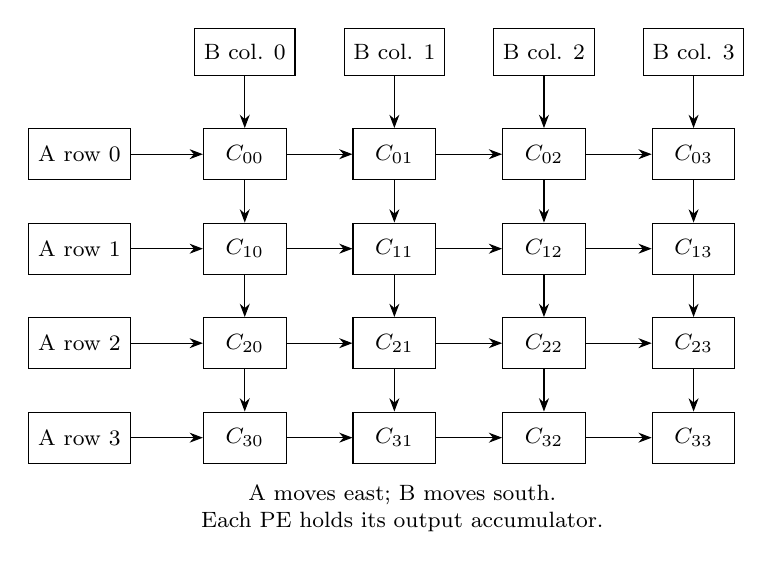
\begin{tikzpicture}[>=Stealth,font=\footnotesize,pe/.style={draw,minimum width=1.05cm,minimum height=.65cm}]
\foreach \i in {0,1,2,3} {
 \foreach \j in {0,1,2,3} {
  \node[pe] (p\i\j) at (1.9*\j,-1.2*\i) {$C_{\i\j}$};
 }
}
\foreach \i in {0,1,2,3} {
 \foreach \j in {0,1,2} {
  \pgfmathtruncatemacro{\next}{\j+1}
  \draw[->] (p\i\j.east)--(p\i\next.west);
  \draw[->] (p\j\i.south)--(p\next\i.north);
 }
 \node[draw,minimum width=1.3cm,minimum height=.65cm] (a\i) at (-2.1,-1.2*\i) {A row \i};
 \draw[->] (a\i)--(p\i0);
 \node[draw,minimum width=1.2cm,minimum height=.6cm] (b\i) at (1.9*\i,1.3) {B col. \i};
 \draw[->] (b\i)--(p0\i);
}
\node[align=center] at (2,-4.5) {A moves east; B moves south.\\Each PE holds its output accumulator.};
\end{tikzpicture}

\caption{The configured 4 by 4 array. Operand packets advance one neighbor per cycle and output accumulators remain in their processing elements.}\label{fig:architecture}
\end{figure}

\section{Correctness and Latency}
The driver generates input matrices with seed 1234 and compares every output against a scalar matrix multiplication. The $4\times4$ result matches and takes 11 calls to the cycle routine. The first call loads the boundary inputs; no PE performs a MAC in that call.

For an $N\times N$ array with the same timing convention, PE $(i,j)$ finishes on call $N+i+j+1$. The last PE therefore finishes on call
\[
L=3N-1.
\]
The operation performs $N^3$ MACs on $N^2$ PEs. Average throughput and utilization are
\[
R=\frac{N^3}{3N-1}\text{ MAC/cycle},\qquad
U=\frac{R}{N^2}=\frac{N}{3N-1}.
\]
\begin{table}[H]\centering\small
\begin{tabular}{lrrrr}
\toprule
N & Cycles & MAC/cycle & Util. \% & Input B/cycle \\
\midrule
4 & 11 & 5.82 & 36.36 & 2.91 \\
16 & 47 & 87.15 & 34.04 & 10.89 \\
64 & 191 & 1372.48 & 33.51 & 42.89 \\
256 & 767 & 21873.81 & 33.38 & 170.89 \\
\bottomrule\end{tabular}\caption{Scaling calculated from the latency model. Only the $4\times4$ case was checked by execution.}\end{table}

\begin{figure}[H]\centering
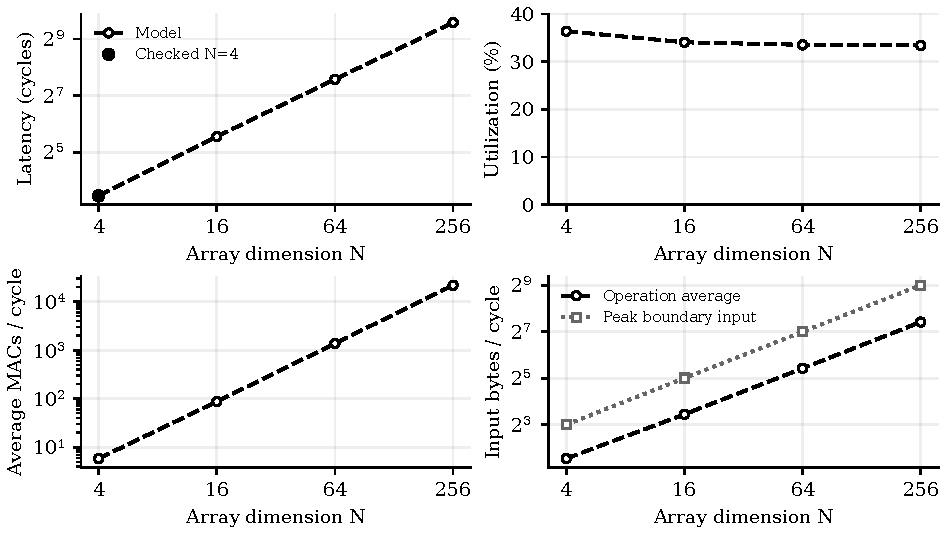
\includegraphics[width=\linewidth]{figures/analytical_scaling.pdf}
\caption{Calculated single-product scaling with $L=3N-1$. Only the filled latency point at $N=4$ was checked by execution. Input bandwidth assumes one-byte elements and excludes output transfer.}\label{fig:results}
\end{figure}

The larger rows are calculated from the latency model. Utilization approaches one third for one product because fill and drain time are included. N is defined in the driver, PE, and FIFO files and must agree across them.

\section{Storage and Bandwidth}
There are $N$ FIFOs on each of two boundaries, each holding $N$ integers. Their data storage is $2N^2\operatorname{sizeof}(int)$ bytes, excluding queue metadata. The array also stores $N^2$ accumulators and the operand packets.

Assuming one-byte operands, loading A and B requires $2N^2$ bytes. The table gives average input bandwidth, $2N^2/(3N-1)$ bytes per cycle, excluding output transfer. Peak boundary input bandwidth can reach $2N$ bytes per cycle. The peak bandwidth curve uses this quantity. The simulator itself stores operands as C integers and does not model an off-chip bandwidth limit.

With one-byte elements, arithmetic intensity is $N/2$ MAC/byte for inputs alone and $N/3$ including output writes. Counting a MAC as two operations doubles both values. These byte counts are modeling assumptions; the program stores integers.


\end{document}
